\chapter{วิศวกรรมปุ๋ยหมัก การย่อยสลายลิกโนเซลลูโลส และพลังงานชีวภาพ}
\label{ch:waste_bioenergy}

\begin{keyconcept}[แนวคิดสำคัญของบทที่ 8]
ของเสียและผลพลอยได้ทางการเกษตร เช่น ฟางข้าว ชานอ้อย ทะลายปาล์ม และมูลสัตว์ เป็นชีวมวลที่มีสารประกอบลิกโนเซลลูโลส (Lignocellulose)\index{สารประกอบลิกโนเซลลูโลส (Lignocellulose)} เป็นองค์ประกอบหลัก ซึ่งทนทานต่อการย่อยสลายทางชีวภาพ การประยุกต์ใช้เอนไซม์จากจุลินทรีย์ (Cellulases, Xylanases, Laccases)\index{เอนไซม์เซลลูเลส (Cellulase Complex)}\index{เอนไซม์แลคเคส (Laccase)} ร่วมกับการควบคุมสภาวะทางวิศวกรรม สามารถเปลี่ยนของเสียเหล่านี้ให้กลายเป็นปุ๋ยอินทรีย์ปรับปรุงดินและพลังงานทดแทน การทำปุ๋ยหมัก (Composting)\index{การทำปุ๋ยหมัก (Composting)} อาศัยการสืบทอดสังคมจุลินทรีย์ (Microbial Succession)\index{การสืบทอดสังคมจุลินทรีย์ (Microbial Succession)} ในสภาวะมีออกซิเจนที่อุณหภูมิสูงกว่า 55\degree C เพื่อทำลายเชื้อโรคและวัชพืช ขณะที่กระบวนการย่อยสลายไร้ออกซิเจน (Anaerobic Digestion: AD)\index{การย่อยสลายไร้ออกซิเจน (Anaerobic Digestion)} อาศัยการทำงานประสานกันของแบคทีเรียและอาร์เคียสร้างมีเทน 4 ขั้นตอน ซึ่งสามารถทำนายอัตราการผลิตก๊าซชีวภาพได้อย่างแม่นยำด้วยแบบจำลอง Modified Gompertz Model\index{แบบจำลอง Modified Gompertz (Modified Gompertz Model)}
\end{keyconcept}

\begin{figure}[ht]
    \centering
    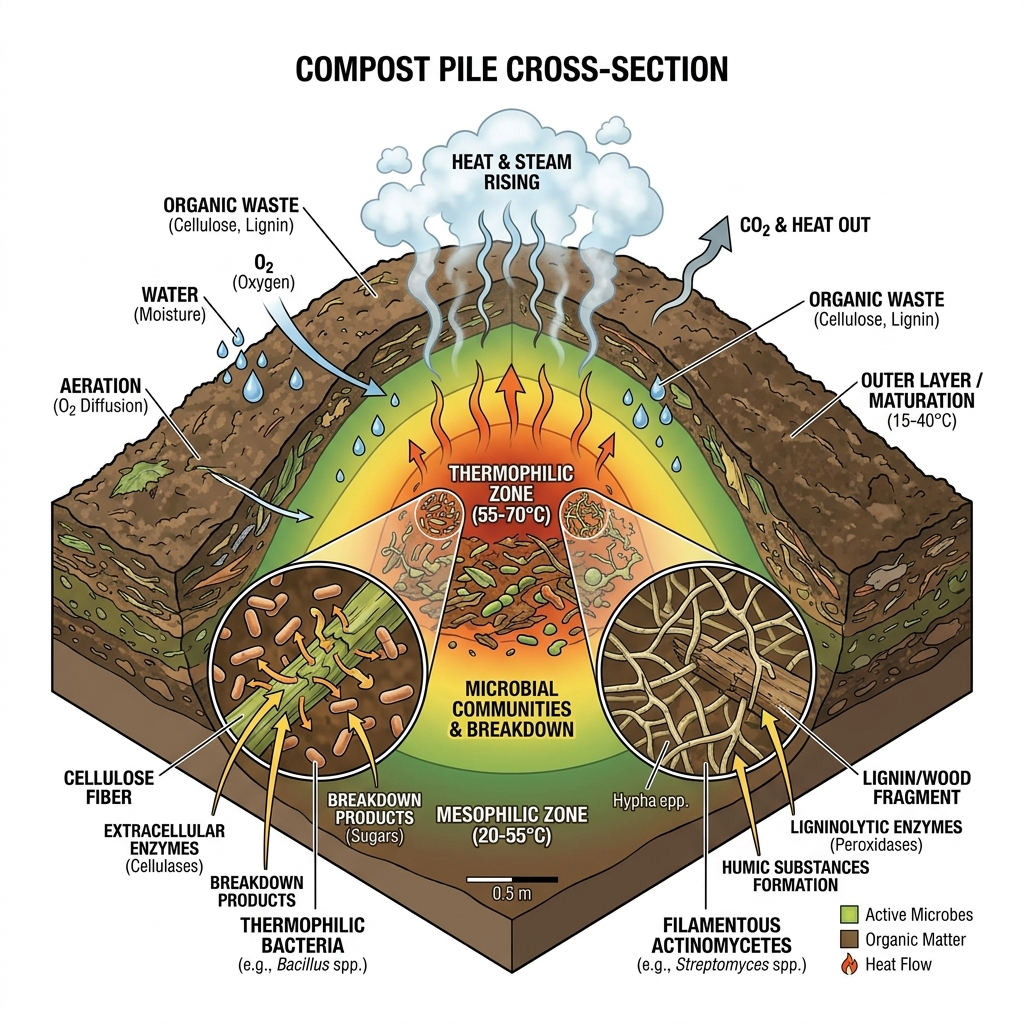
\includegraphics[width=0.85\textwidth]{assets/ch08_composting_microbes.png}
    \caption{การจำลอง 3D แสดงการสืบทอดทางนิเวศวิทยาของจุลินทรีย์ในกองปุ๋ยหมัก (Compost microbial succession) แสดงการเปลี่ยนผ่านจากระยะเริ่มต้นอุณหภูมิปานกลาง (Mesophilic) สู่ระยะอุณหภูมิสูง (Thermophilic phase) ซึ่งแบคทีเรียทนร้อนและแอคติโนมัยซีสย่อยสลายสารอินทรีย์อย่างรวดเร็ว ทำลายเชื้อก่อโรคพืช ก่อนลดอุณหภูมิลงสู่ระยะบ่มตัว (Curing phase)}
    \label{fig:ch08_composting_microbes}
\end{figure}

\section*{วัตถุประสงค์การเรียนรู้ประจำบท}
เมื่อศึกษาบทเรียนนี้จบแล้ว นักศึกษาสามารถ:
\begin{enumerate}
    \item อธิบายโครงสร้างระดับโมเลกุลของลิกโนเซลลูโลส และระบบเอนไซม์ย่อยสลายของจุลินทรีย์ (Cellulase complex และ Lignin-modifying enzymes)
    \item วิเคราะห์พลวัตการสืบทอดของประชากรจุลินทรีย์ทั้ง 4 ระยะในกระบวนการทำปุ๋ยหมักแบบใช้ออกซิเจน
    \item คำนวณระบบสมการดุลมวลสารเพื่อปรับอัตราส่วน C:N และความชื้นของกองปุ๋ยหมักให้ได้เกณฑ์มาตรฐาน
    \item อธิบาย 4 ขั้นตอนเคมีชีวภาพของการย่อยสลายไร้ออกซิเจน (Hydrolysis, Acidogenesis, Acetogenesis, Methanogenesis)
    \item คำนวณและทำนายผลผลิตก๊าซมีเทนสะสมด้วยแบบจำลองจลนศาสตร์ Modified Gompertz Model
\end{enumerate}

\section{ชีวเคมีของการย่อยสลายสารประกอบลิกโนเซลลูโลส}

ชีวมวลพืชประกอบด้วยโครงสร้างพอลิเมอร์ธรรมชาติที่สลับซับซ้อน 3 ชนิดที่ประสานกันอย่างเหนียวแน่น เรียกว่า **ลิกโนเซลลูโลส (Lignocellulose)**:
\begin{enumerate}
    \item \textbf{เซลลูโลส (Cellulose, 40--50\%):} สายพอลิเมอร์เส้นตรงของกลูโคสที่เชื่อมกันด้วยพันธะ $\beta$-1,4-glycosidic ยึดเหนี่ยวกันด้วยพันธะไฮโดรเจนกลายเป็นเส้นใยไมโครไฟบริล (Microfibrils) ที่มีทั้งบริเวณอสัณฐาน (Amorphous) และบริเวณผลึกแน่น (Crystalline region)
    \item \textbf{เฮมิเซลลูโลส (Hemicellulose, 25--35\%):} พอลิแซ็กคาไรด์สายกิ่งที่ประกอบด้วยน้ำตาลเพนโทส (Xylose, Arabinose) และเฮกโซส (Mannose, Galactose, Glucose)
    \item \textbf{ลิกนิน (Lignin, 15--25\%):} พอลิเมอร์อสัณฐานไม่สม่ำเสมอของสารประกอบฟีนอลิก (Phenylpropane units) 3 ชนิด ได้แก่ $p$-coumaryl alcohol, coniferyl alcohol, และ sinapyl alcohol เชื่อมกันด้วยพันธะอีเทอร์ (Ether bonds: $\beta$-O-4) และพันธะคาร์บอน-คาร์บอน (C-C) ที่ทนทานต่อการย่อยสลายทางเคมีมากที่สุด
\end{enumerate}

\subsection{ระบบเอนไซม์ย่อยสลายลิกโนเซลลูโลสของจุลินทรีย์}
\begin{itemize}
    \item \textbf{ระบบเอนไซม์เซลลูเลส (Cellulase Enzyme Complex):} ประกอบด้วยเอนไซม์ 3 ชนิดที่ทำงานเสริมฤทธิ์กัน:
    \begin{enumerate}
        \item \textit{Endo-$\beta$-1,4-glucanase (EC 3.2.1.4):} สุ่มตัดพันธะภายในสายเซลลูโลสบริเวณอสัณฐาน สร้างปลายสายอิสระ
        \item \textit{Exo-$\beta$-1,4-glucanase หรือ Cellobiohydrolase (EC 3.2.1.91):} ตัดน้ำตาลไดแซ็กคาไรด์ **เซลโลไบโอส (Cellobiose)** ออกจากปลายสายอย่างต่อเนื่อง
        \item \textit{$\beta$-Glucosidase (EC 3.2.1.21):} ย่อยสลายเซลโลไบโอสให้กลายเป็นน้ำตาลกลูโคสอิสระ
    \end{enumerate}
    \item \textbf{เอนไซม์ย่อยลิกนิน (Lignin-Modifying Enzymes: LMEs):} พบเด่นชัดในเชื้อรากลุ่มผุขาว (White-rot fungi: เช่น \organism{Phanerochaete chrysosporium}\index{Phanerochaete chrysosporium@\textit{Phanerochaete chrysosporium}}, \organism{Pleurotus ostreatus}\index{Pleurotus ostreatus@\textit{Pleurotus ostreatus}}):
    \begin{itemize}
        \item \textbf{Laccase (EC 1.10.3.2):} เอนไซม์ที่มีทองแดงเป็นองค์ประกอบ ใช้ออกซิเจน ($O_2$) ออกซิไดซ์หมู่วงแหวนฟีนอลของลิกนิน\index{เอนไซม์แลคเคส (Laccase)}
        \item \textbf{Lignin Peroxidase (LiP, EC 1.11.1.14)\index{Lignin Peroxidase (LiP)} และ Manganese Peroxidase (MnP, EC 1.11.1.13):\index{Manganese Peroxidase (MnP)}} เอนไซม์กลุ่มฮีม (Heme-peroxidases) ที่อาศัยไฮโดรเจนเปอร์ออกไซด์ ($H_2O_2$) สร้างอนุมูลอิสระที่มีพลังออกซิเดชันสูงมาก สามารถตัดพันธะ $\beta$-O-4 ของลิกนินที่ไม่มีหมู่ฟีนอลได้
    \end{itemize}
\end{itemize}

\section{วิศวกรรมการทำปุ๋ยหมักและการสืบทอดสังคมจุลินทรีย์}

กระบวนการทำปุ๋ยหมักแบบใช้ออกซิเจน (Aerobic Composting) เป็นการสลายตัวของสารอินทรีย์โดยจุลินทรีย์จนได้ผลิตภัณฑ์ที่มีความเสถียร (Humus) โดยอุณหภูมิภายในกองปุ๋ยจะเปลี่ยนแปลงตามกิจกรรมเมแทบอลิซึม ซึ่งแบ่งออกเป็น 4 ระยะ:

\begin{figure}[ht]
\centering
\resizebox{0.96\textwidth}{!}{
\begin{tikzpicture}
    % Axes
    \draw[->, thick] (0,0) -- (11.5,0) node[right] {\small \textbf{เวลา (วัน)}};
    \draw[->, thick] (0,0) -- (0,6.5) node[above] {\small \textbf{อุณหภูมิ (\degree C)}};
    
    % Temperature ticks
    \draw (0,2) node[left] {\small 25\degree C};
    \draw (0,3.6) node[left] {\small 45\degree C};
    \draw (0,4.8) node[left] {\small 60\degree C};
    
    % Safe sanitation line
    \draw[dashed, red, thick] (0,4.4) -- (11.0,4.4);
    \node[red, font=\scriptsize\bfseries, above] at (5.5, 4.4) {เกณฑ์ทำลายเชื้อโรคพืช ($\ge 55^\circ\text{C}$)};
    
    % Temperature curve
    \draw[line width=2.0pt, earthbrown] 
        (0,1.8) .. controls (1.5,2.5) and (2.0,3.5) .. 
        (3.0,5.2) .. controls (4.5,5.6) and (5.5,5.4) .. 
        (7.0,4.0) .. controls (8.5,2.8) and (10.0,2.2) .. (11.0,2.0);
        
    % Phase regions
    \draw[dashed, gray] (2.2,0) -- (2.2,6);
    \draw[dashed, gray] (6.5,0) -- (6.5,6);
    \draw[dashed, gray] (9.0,0) -- (9.0,6);
    
    % Phase labels
    \node[align=center] at (1.1,5.8) {\small \textbf{ระยะที่ 1}\\Mesophilic};
    \node[align=center] at (4.35,6.2) {\small \textbf{ระยะที่ 2}\\Thermophilic};
    \node[align=center] at (7.75,5.8) {\small \textbf{ระยะที่ 3}\\Cooling};
    \node[align=center] at (10.0,5.8) {\small \textbf{ระยะที่ 4}\\Curing};
\end{tikzpicture}
}
\caption{กราฟพลวัตอุณหภูมิและการเปลี่ยนผ่านประชากรจุลินทรีย์ 4 ระยะในกระบวนการทำปุ๋ยหมักแบบกองใช้ออกซิเจน}
\label{fig:compost_temp_profile}
\end{figure}

\begin{enumerate}
    \item \textbf{ระยะอุณหภูมิปานกลางเริ่มต้น (Mesophilic Phase, 20--45\degree C):} เกิดขึ้นใน $1 - 3\text{ วันแรก}$ จุลินทรีย์กลุ่มมีโซไฟล์ (แบคทีเรีย ยีสต์) ย่อยสลายน้ำตาล แป้ง และกรดอะมิโนอย่างรวดเร็ว ปลดปล่อยความร้อนสะสม
    \item \textbf{ระยะอุณหภูมิสูง (Thermophilic Phase, 45--65\degree C):\index{ระยะอุณหภูมิสูง (Thermophilic Phase)}} แบคทีเรียทนร้อน เช่น \organism{Bacillus stearothermophilus}, \organism{Thermus} spp. และแอคติโนมัยซีสทนร้อน เช่น \organism{Thermoactinomyces vulgaris} เข้าทำหน้าที่ย่อยสลายเซลลูโลสและโปรตีน 
    \begin{itemize}
        \item \textbf{เกณฑ์ความปลอดภัยทางชีวภาพ (Sanitation Standard):\index{เกณฑ์ความปลอดภัยทางชีวภาพ (Sanitation Standard)}} กองปุ๋ยต้องมีอุณหภูมิสูงกว่า $55^\circ\text{C}$ ต่อเนื่องกันอย่างน้อย 3 วัน (ในระบบท่อเติมอากาศ) หรืออย่างน้อย 15 วันพร้อมพลิกกอง 5 ครั้ง (ในระบบกองแถวยาว: Windrow) เพื่อทำลายเชื้อก่อโรคพืช ไข่พยาธิ และเมล็ดวัชพืชให้หมดสิ้น
    \end{itemize}
    \item \textbf{ระยะลดอุณหภูมิ (Cooling Phase):} เมื่อสารอินทรีย์ที่ย่อยง่ายหมดลง ความร้อนลดลง เชื้อราสายใยทนแล้งจะกลับเข้าย่อยเซลลูโลสและลิกนินที่หลงเหลือ
    \item \textbf{ระยะบ่มตัว (Curing / Maturation Phase):} สังคมจุลินทรีย์สังเคราะห์สารฮิวมัส (Humic and Fulvic acids) ดัชนี C:N ลดลงต่ำกว่า $15:1$ ปุ๋ยมีความเสถียรและไม่มีสารพิษต่อการงอกของเมล็ด (Phytotoxin-free)
\end{enumerate}

\section{วิศวกรรมการผลิตก๊าซชีวภาพ (Anaerobic Digestion)}

กระบวนการย่อยสลายสารอินทรีย์แบบไร้ออกซิเจน (Anaerobic Digestion: AD)\index{การย่อยสลายไร้ออกซิเจน (Anaerobic Digestion)} ประกอบด้วย 4 ขั้นตอนทางชีวเคมีที่ทำงานต่อเนื่องกันเป็นลูกโซ่:

\begin{figure}[ht]
\centering
\begin{tikzpicture}[node distance=1.6cm, auto,
    block/.style={rectangle, draw, fill=cyan!15, text width=9.5cm, rounded corners, minimum height=1.0cm, align=left},
    arrow/.style={thick, ->, >=stealth}]
    
    \node [block] (step1) {\textbf{1. ไฮโดรไลซิส (Hydrolysis):} คาร์โบไฮเดรต, โปรตีน, ลิพิด $\xrightarrow{\text{Enzymes}}$ น้ำตาล, กรดอะมิโน, กรดไขมัน};
    \node [block, below of=step1] (step2) {\textbf{2. แอซิโดเจเนซิส (Acidogenesis):} น้ำตาล, กรดอะมิโน $\xrightarrow{\text{Acidogens}}$ กรดไขมันระเหยง่าย (VFAs), แอลกอฮอล์, $H_2, CO_2$};
    \node [block, below of=step2] (step3) {\textbf{3. อะซิโตเจเนซิส (Acetogenesis):} กรดบิวทีริก, กรดโพรพิโอนิก $\xrightarrow{\text{Acetogens}}$ กรดอะซิติก ($CH_3COOH$), $H_2, CO_2$};
    \node [block, below of=step3] (step4) {\textbf{4. มีเทนโนเจเนซิส (Methanogenesis):} $CH_3COOH, H_2, CO_2 \xrightarrow{\text{Methanogens}}$ ก๊าซมีเทน ($CH_4$) + $CO_2$};
    
    \draw [arrow] (step1) -- (step2);
    \draw [arrow] (step2) -- (step3);
    \draw [arrow] (step3) -- (step4);
\end{tikzpicture}
\caption{ลำดับขั้นชีวเคมี 4 ขั้นตอนในกระบวนการผลิตก๊าซชีวภาพไร้ออกซิเจน}
\label{fig:ad_steps}
\end{figure}

\subsection{1. วิถีการสังเคราะห์ก๊าซมีเทน (Methanogenic Pathways)}
\begin{itemize}
    \item \textbf{Acetoclastic Pathway (ร้อยละ 65--70 ของมีเทนทั้งหมด):}
    \begin{equation}
    CH_3COOH \longrightarrow CH_4 + CO_2 \quad (\Delta G^\circ = -31.0\text{ kJ/mol})
    \end{equation}
    ดำเนินการโดยอาร์เคียสกุล \organism{Methanosaeta}\index{Methanosaeta@\textit{Methanosaeta}} (ชอบความเข้มข้นอะซิเตตต่ำ) และ \organism{Methanosarcina}\index{Methanosarcina@\textit{Methanosarcina}} (เติบโตเร็วที่อะซิเตตสูง)
    \item \textbf{Hydrogenotrophic Pathway (ร้อยละ 30 ของมีเทนทั้งหมด):}
    \begin{equation}
    CO_2 + 4 H_2 \longrightarrow CH_4 + 2 H_2O \quad (\Delta G^\circ = -131.0\text{ kJ/mol})
    \end{equation}
    ดำเนินการโดยอาร์เคียสกุล \organism{Methanoculleus} และ \organism{Methanobrevibacter}
\end{itemize}

\subsection{2. เสถียรภาพของบ่อหมักและอัตราส่วน VFA/Alkalinity (Ripley Ratio)}
กลุ่ม Acidogens เติบโตได้เร็วกว่ากลุ่ม Methanogens ถึง 10 เท่า หากป้อนสารอาหารมากเกินไป กรดไขมันระเหยง่าย (VFAs) จะสะสมจนค่า pH ลดต่ำกว่า 6.5 ซึ่งจะยับยั้ง Methanogens ทันที ทำให้บ่อหมักเน่าเสีย (Soured digester) ผู้ควบคุมระบบต้องติดตามอัตราส่วน:
$$\text{Ripley Ratio}\index{อัตราส่วน Ripley (Ripley Ratio)} = \frac{\text{VFA (mg/L)}}{\text{Alkalinity (mg } CaCO_3\text{/L)}} < 0.3 \text{ (สภาวะปกติเสถียร)}$$
หากอัตราส่วนเกิน 0.4 บ่งชี้ว่าระบบกำลังเข้าสู่ภาวะวิกฤติต้องหยุดป้อนของเสียและเติมปูนขาวหรือด่างทันที

\subsection{3. แบบจำลอง Modified Gompertz Model}
การทำนายปริมาณก๊าซมีเทนสะสม ($B(t)$) จากการทดสอบความสามารถในการสร้างก๊าซชีวภาพ (Biochemical Methane Potential: BMP) นิยมใช้แบบจำลองทางคณิตศาสตร์ที่ไม่เป็นเชิงเส้น **Modified Gompertz Model**:

\begin{equation}
B(t) = P \cdot \exp\left\{ - \exp\left[ \frac{R_m \cdot e}{P} (\lambda - t) + 1 \right] \right\}
\end{equation}

เมื่อ:
\begin{itemize}
    \item $B(t)$ คือปริมาณก๊าซมีเทนสะสม ณ เวลา $t$ ($\text{mL } CH_4/\text{g VS}$)
    \item $P$ คือศักยภาพผลผลิตก๊าซมีเทนสูงสุด (Methane yield potential, $\text{mL } CH_4/\text{g VS}$)
    \item $R_m$ คืออัตราการสร้างก๊าซมีเทนสูงสุด (Maximum methane production rate, $\text{mL } CH_4/\text{g VS}\cdot\text{day}$)
    \item $\lambda$ คือระยะหน่วงเวลาเริ่มต้น (Lag phase duration, วัน)
    \item $e$ คือค่าคงที่ออยเลอร์ ($e \approx 2.71828$)
    \item $t$ คือระยะเวลาการหมัก (วัน)
\end{itemize}

\begin{worked}[ตัวอย่างที่ 8.1 การคำนวณสัดส่วนผสมวัสดุทำปุ๋ยหมักเพื่อปรับ C:N Ratio และความชื้น]
โรงงานผลิตปุ๋ยอินทรีย์ต้องการผสม **ฟางข้าวสับแห้ง (วัสดุ 1)** ร่วมกับ **มูลไก่เนื้อสด (วัสดุ 2)** เพื่อเตรียมกองปุ๋ยหมักน้ำหนักแห้งรวม $1,000\text{ kg}$ โดยกำหนดให้กองปุ๋ยหมักเริ่มต้นมีอัตราส่วน $\text{C:N} = 30:1$ 

คุณสมบัติทางเคมีของวัสดุ (คิดบนฐานน้ำหนักแห้ง):
\begin{itemize}
    \item ฟางข้าวสับ: คาร์บอน $C_1 = 45\%$, ไนโตรเจน $N_1 = 0.6\%$, ความชื้น $M_1 = 12\%$
    \item มูลไก่เนื้อสด: คาร์บอน $C_2 = 36\%$, ไนโตรเจน $N_2 = 3.6\%$, ความชื้น $M_2 = 70\%$
\end{itemize}
จงคำนวณหาน้ำหนักแห้ง ($W_1$ และ $W_2$) และน้ำหนักสดของวัสดุทั้งสองที่ต้องนำมาผสมกัน

\textbf{วิธีทำ:}
1. กำหนดระบบสมการเชิงเส้น:
สมการมวลรวมน้ำหนักแห้ง:
$$W_1 + W_2 = 1,000\text{ kg}$$
$$W_2 = 1,000 - W_1$$

สมการดุลอัตราส่วน C:N:
$$\frac{C_{\text{total}}}{N_{\text{total}}} = \frac{0.45 W_1 + 0.36 W_2}{0.006 W_1 + 0.036 W_2} = 30$$
$$0.45 W_1 + 0.36 W_2 = 30 \times (0.006 W_1 + 0.036 W_2)$$
$$0.45 W_1 + 0.36 W_2 = 0.18 W_1 + 1.08 W_2$$
$$(0.45 - 0.18) W_1 = (1.08 - 0.36) W_2$$
$$0.27 W_1 = 0.72 W_2 \implies W_1 = \frac{0.72}{0.27} W_2 \approx 2.667 W_2$$

2. แทนค่าหา $W_2$ และ $W_1$:
$$2.667 W_2 + W_2 = 1,000 \implies 3.667 W_2 = 1,000$$
$$W_2 = \frac{1,000}{3.667} \approx 272.7\text{ kg (น้ำหนักแห้งมูลไก่)}$$
$$W_1 = 1,000 - 272.7 = 727.3\text{ kg (น้ำหนักแห้งฟางข้าว)}$$

3. แปลงเป็นน้ำหนักสด (Wet Weight: $W_{\text{wet}} = W_{\text{dry}} / (1 - M)$):
$$W_{\text{สดฟางข้าว}} = \frac{727.3}{1 - 0.12} = \frac{727.3}{0.88} \approx 826.5\text{ kg}$$
$$W_{\text{สดมูลไก่}} = \frac{272.7}{1 - 0.70} = \frac{272.7}{0.30} \approx 909.0\text{ kg}$$

\textbf{บทวิเคราะห์ผลลัพธ์:} การใช้ฟางข้าวสด $826.5\text{ kg}$ ผสมกับมูลไก่สด $909.0\text{ kg}$ จะได้กองปุ๋ยที่มีสัดส่วน C:N เท่ากับ $30:1$ อย่างสมบูรณ์แบบ ซึ่งเป็นสัดส่วนที่ให้พลังงานคาร์บอนและไนโตรเจนที่สมดุลแก่แบคทีเรียทนร้อน ทำให้กองปุ๋ยมีอุณหภูมิพุ่งขึ้นสู่ระยะ Thermophilic ได้อย่างรวดเร็ว
\end{worked}

\begin{worked}[ตัวอย่างที่ 8.2 การประยุกต์ใช้แบบจำลอง Modified Gompertz ทำนายผลผลิตก๊าซมีเทน]
จากการหมักชานอ้อยร่วมกับมูลวัวในถังหมักแบบกะขนาดกึ่งอุตสาหกรรม นักวิจัยวิเคราะห์พารามิเตอร์ของ Modified Gompertz Model ได้ดังนี้:
\begin{itemize}
    \item ศักยภาพผลผลิตมีเทนสูงสุด $P = 320\text{ mL } CH_4/\text{g VS}$
    \item อัตราการผลิตสูงสุด $R_m = 18.5\text{ mL } CH_4/\text{g VS}\cdot\text{day}$
    \item ระยะหน่วงเวลาเริ่มต้น $\lambda = 3.5\text{ วัน}$
\end{itemize}
จงคำนวณปริมาณก๊าซมีเทนสะสม $B(t)$ ณ วันที่ 10 ของการหมัก

\textbf{วิธีทำ:}
แทนค่า $t = 10$ ลงในสมการ Modified Gompertz:
$$B(10) = 320 \cdot \exp\left\{ - \exp\left[ \frac{18.5 \times 2.71828}{320} (3.5 - 10) + 1 \right] \right\}$$

1. คำนวณเทอมภายในวงเล็บ:
$$\frac{18.5 \times 2.71828}{320} = \frac{50.288}{320} \approx 0.15715$$
$$(3.5 - 10) = -6.5$$
$$0.15715 \times (-6.5) = -1.0215$$
$$-1.0215 + 1 = -0.0215$$

2. คำนวณเอกซ์โพเนนเชียลสองชั้น:
$$\exp(-0.0215) \approx 0.9787$$
$$\exp(-0.9787) \approx 0.3758$$

3. คำนวณค่า $B(10)$:
$$B(10) = 320 \times 0.3758 \approx 120.26\text{ mL } CH_4/\text{g VS}$$

\textbf{บทวิเคราะห์ผลลัพธ์:} ณ วันที่ 10 หลังเริ่มเดินระบบ ถังหมักผลิตก๊าซมีเทนสะสมได้ $120.26\text{ mL/g VS}$ หรือคิดเป็น $37.58\%$ ของศักยภาพสูงสุด ข้อมูลนี้ช่วยให้วิศวกรสามารถวางแผนการจ่ายก๊าซชีวภาพเข้าสู่เครื่องกำเนิดไฟฟ้า (Biogas Generator) ได้อย่างแม่นยำ
\end{worked}

% [RESEARCH-UPDATE-2026-10]
\section{ความก้าวหน้างานวิจัยล่าสุดด้านการจัดการของเสียและการหมัก}

รายงานการวิจัยระดับนานาชาติในปี ค.ศ. 2024–2026 โดย Chen และคณะ \cite{pmid37471462} ได้พัฒนาหัวเชื้อจุลินทรีย์ร่วม (Consortium) ของเชื้อรากลุ่มทนร้อน \organism{Aspergillus fumigatus} และแบคทีเรีย \organism{Geobacillus} ที่สามารถเร่งการสลายพันธะลิกโนเซลลูโลสในกองปุ๋ยหมักฟางข้าวได้เร็วกว่าเดิมถึง $40\%$ ส่งผลให้อุณหภูมิสูงขึ้นแตะ $60^\circ\text{C}$ ได้ภายใน 36 ชั่วโมง

ในขณะเดียวกัน งานวิจัยของ Yang และคณะ \cite{pmid40131450} ได้เสนอการประยุกต์ใช้ถ่านชีวภาพร่วมกับแบคทีเรียออกซิไดซ์แอมโมเนีย เพื่อดักจับและอนุรักษ์ก๊าซแอมโมเนีย ($NH_3$) ที่ระเหยออกจากกองปุ๋ยหมัก เปลี่ยนรูปเป็นไนเตรต ($NO_3^-$) ในเนื้อปุ๋ย ซึ่งช่วยลดการสูญเสียไนโตรเจนลงได้ถึง $62\%$ และลดมลพิษทางกลิ่นได้อย่างเด็ดขาด

\begin{insight}[ประเด็นวิเคราะห์เชิงวิชาการ]
ในโรงงานผลิตแป้งมันสำปะหลัง น้ำเสียมีค่ากรดอินทรีย์สูงมาก หากนำเข้าสู่ระบบบ่อหมักก๊าซชีวภาพแบบ CSTR โดยตรง มักทำให้ระบบล่มเนื่องจากค่า pH ดิ่งลงต่ำกว่า 5.5 จงเสนอแนวทางแก้ไขโดยใช้หลักการสองขั้นตอน (Two-Stage Anaerobic Digestion)
\end{insight}

\section*{สรุปประจำบท}

การแปรสภาพของเสียทางการเกษตรให้เป็นปุ๋ยอินทรีย์และพลังงานชีวภาพเป็นกลไกขับเคลื่อนหลักของเศรษฐกิจหมุนเวียน (Circular Bioeconomy) การย่อยสลายลิกโนเซลลูโลสต้องอาศัยการทำงานประสานกันของเอนไซม์ Endoglucanase, Exoglucanase, $\beta$-Glucosidase และเอนไซม์ดัดแปรลิกนิน Laccase/Peroxidases การทำปุ๋ยหมักต้องควบคุมสัดส่วน C:N (25--30:1) และความชื้น (50--60\%) เพื่อสนับสนุนการสืบทอดของประชากรจุลินทรีย์ในระยะ Thermophilic ($> 55^\circ\text{C}$) เพื่อทำลายเชื้อก่อโรคอย่างสมบูรณ์ สำหรับการผลิตก๊าซชีวภาพ การรักษาสมดุลระหว่าง Acidogens และ Methanogens โดยควบคุมอัตราส่วน Ripley Ratio ($< 0.3$) ควบคู่กับการใช้แบบจำลอง Modified Gompertz ช่วยให้การบริหารจัดการพลังงานทดแทนในภาคการเกษตรเป็นไปอย่างมีประสิทธิภาพสูงสุด

\subsection*{คำถามท้ายบทและการวิเคราะห์}

\noindent \textbf{ระดับที่ 1: ความรู้และความเข้าใจเชิงทฤษฎี (Knowledge \& Comprehension)}
\begin{enumerate}
    \item อธิบายโครงสร้างโมเลกุลของลิกโนเซลลูโลส และระบุว่าสารประกอบใดเป็นอุปสรรคสำคัญที่สุดต่อการย่อยสลายของจุลินทรีย์ เพราะเหตุใด?
    \item สรุปหน้าที่ของเอนไซม์ 3 ชนิดใน Cellulase Complex ในการย่อยสลายเส้นใยเซลลูโลสให้เป็นน้ำตาลกลูโคส
    \item อธิบายความสำคัญของการคงอุณหภูมิที่สูงกว่า 55\degree C ต่อเนื่องกันอย่างน้อย 3 วันในกองปุ๋ยหมัก
    \item อธิบายลำดับขั้นตอนชีวเคมี 4 ขั้นตอนของการย่อยสลายสารอินทรีย์ไร้ออกซิเจน (Anaerobic Digestion)
\end{enumerate}

\noindent \textbf{ระดับที่ 2: การวิเคราะห์และการคำนวณเชิงปริมาณ (Quantitative Analysis \& Calculation)}
\begin{enumerate}[resume]
    \item เปรียบเทียบความแตกต่างระหว่าง Acetoclastic Methanogenesis และ Hydrogenotrophic Methanogenesis ในแง่ของสัดส่วนก๊าซมีเทนที่ผลิตได้และชนิดของอาร์เคียที่เกี่ยวข้อง
    \item ค่า Ripley Ratio (VFA/Alkalinity) มีความสำคัญอย่างไรในการเฝ้าระวังความผิดปกติของบ่อหมักก๊าซชีวภาพ?
    \item ต้องการผสมเศษเปลือกผลไม้ ($C = 40\%$, $N = 1\%$, ความชื้น $80\%$) กับแกลบแห้ง ($C = 42\%$, $N = 0.3\%$, ความชื้น $10\%$) เพื่อให้ได้อัตราส่วน C:N เริ่มต้น $28:1$ บนฐานน้ำหนักแห้งรวม $500\text{ kg}$ จงคำนวณหาน้ำหนักแห้งของวัสดุแต่ละชนิด
\end{enumerate}

\noindent \textbf{ระดับที่ 3: การสังเคราะห์และการแก้ปัญหาในแปลงจริง (Application \& Real-World Synthesis)}
\begin{enumerate}[resume]
    \item ในกระบวนการทำปุ๋ยหมักระยะบ่มตัว (Curing Phase) เกิดการเปลี่ยนแปลงทางชีวเคมีใดบ้างที่ทำให้ปุ๋ยหมักปลอดภัยต่อการนำไปใช้เพาะปลูก?
    \item อธิบายความหมายเชิงฟิสิกส์ของตัวแปร $P$, $R_m$ และ $\lambda$ ในสมการ Modified Gompertz Model และการนำไปใช้วางแผนจ่ายก๊าซในฟาร์ม
    \item ออกแบบผังระบบบำบัดน้ำเสียฟาร์มสุกรแบบบูรณาการ ที่สามารถผลิตก๊าซชีวภาพ บำบัดน้ำทิ้งด้วยจุลินทรีย์สังเคราะห์แสง (PSB) และนำตะกอนเลนมาทำปุ๋ยหมักชีวภาพ
\end{enumerate}
